\documentclass{report}
\usepackage{homework}
\solstrue

\usepackage{graphicx}
\graphicspath{{figures/}}

\renewcommand{\hmwkTitle}{Homework 4}

\begin{document}
\mktitle

\begin{problem}

Host A sends 5 data segments to Host B, the 2nd segment (sent from A) is lost. This loss is then detected by the protocol-specific means and the protocol invokes recovery actions. In the end, all 5 data segments are correctly received by Host B.

\begin{enumerate}
\item If A and B use Go-back-N for the data delivery, what is the total number of segments that Host A sent out (including retransmissions)? And what is the total number ACKs that Host B sent?

\item If A and B use TCP for the data delivery (no delayed ACKs), what is the total number of segments that Host A sent out (including retransmissions)? And what is the total number ACKs that Host B sent?

\item Assume that the retransmission timer is set to 10*RTT, which of the above two protocols (Go-back-N and TCP) finish the data delivery first?
\end{enumerate}
Note: Answering questions 2 and 3 requires the knowledge about TCP fast retransmit, which is described on Lecture-7, slides 24-25, that will be discussed in next Monday lecture. If anyone wants to finish the homework this weekend, you probably can figure out how TCP fast retransmit works by taking a careful look at Lecture-7, slides 24-25.

\begin{answer}{40em}
    Write your answer here
\end{answer}

\end{problem}



\newpage



\begin{problem}

Host A and B are communicating over a TCP connection, and Host B has
already received from A all bytes up through byte 126. Suppose Host A then
sends two segments to Host B back-to-back. The first and second segments
contain 80 and 40 bytes of data, respectively. In the first segment, the
sequence number is 127, the source port number is 302, and the destination
port number is 80. Host B sends an acknowledgment whenever it receives a
segment from Host A.

\begin{enumerate}
\item In the second segment sent from Host A to B, what are the sequence number, source port number, and destination port number?

\item If the first segment arrives before the second segment, in the acknowledgment of the first arriving segment, what is the acknowledgment number, the source port number, and the destination port number?

\item If the second segment arrives before the first segment, in the acknowledgment of the first arriving segment, what is the acknowledgment number?

\end{enumerate}

\begin{answer}{40em}
    Write your answer here
\end{answer}

\end{problem}

\newpage

\begin{problem}
Follow the same problem setting in Page 37 of Slides lecture-06. Suppose packet size is 4000 bits, bandwidth is 2Mbps, and propagation delay is 15 msec. Ignore packet loss.

\begin{enumerate}
\item Suppose window size is 10, will the sender be kept busy? If yes, explain why. If not, What is the effective throughput? 
\item What is the minimum window size to achieve full utilization? Then how many bits would be needed for the sequence number field?
\end{enumerate}

\begin{answer}{35em}
  Write your answer here
\end{answer}

\end{problem}


\newpage


\begin{problem}
Consider a reliable data transfer protocol that uses only negative acknowledgments. Suppose the sender has a lot of data to send and the end-to-end connection experiences few losses. Would a NAK-only protocol be preferable to a protocol that uses ACKs? Why? Now suppose the sender sends data only infrequently. In this second case, would a NAK-only protocol be preferable to a protocol that uses ACKs? Why? \\

\begin{answer}{35em}
  Write your answer here
\end{answer}

\end{problem}

\newpage



\begin{problem}

A sends a TCP FIN message to B to close the TCP connection with B, the TCP header of A's FIN message is shown below. 
When B receives A's TCP FIN, it also decides to close the connection, so B sends a combined FIN and FIN-ACK message, whose TCP header is also shown below.  Please fill in all the fields with a question mark in this TCP header.

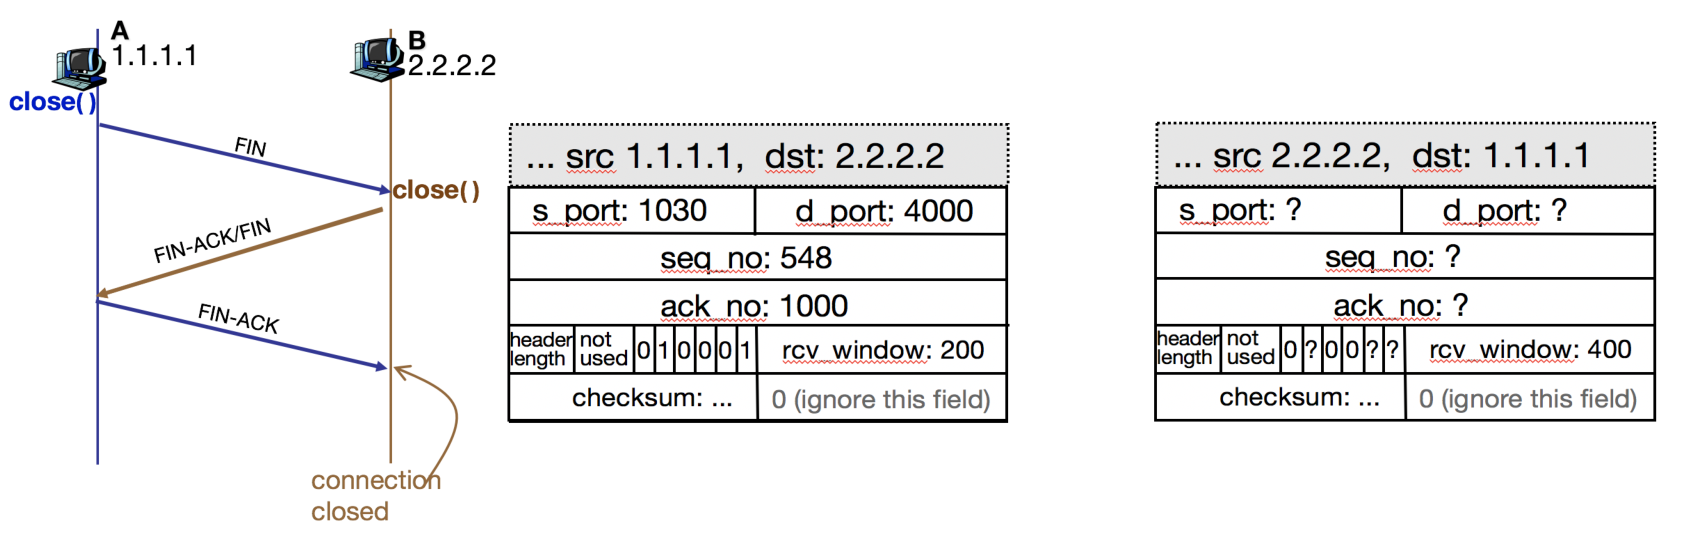
\includegraphics[width=\textwidth]{hw4_fig.pdf}

\begin{answer}{35em}

    \texttt{s\_port:}  \\
    \texttt{d\_port:}  \\
    \texttt{seq\_no:}  \\
    \texttt{ack\_no:}  \\
    \texttt{control bits (6-bit):}  \\
\end{answer}

\end{problem}

\end{document}
